%%%%%%%%%%%%%%%%%%%%%%%%%%%%%%%%%%%
%This is the LaTeX ARTICLE template for RSC journals
%Copyright The Royal Society of Chemistry 2016
%%%%%%%%%%%%%%%%%%%%%%%%%%%%%%%%%%%

\documentclass[twoside,twocolumn,9pt]{article}
\usepackage{extsizes}
\usepackage[super,sort&compress,comma]{natbib} 
\usepackage[version=3]{mhchem}
\usepackage[left=1.5cm, right=1.5cm, top=1.785cm, bottom=2.0cm]{geometry}
\usepackage{balance}
\usepackage{mathptmx}
\usepackage{sectsty}
\usepackage{graphicx} 
\usepackage{lastpage}
\usepackage[format=plain,justification=justified,singlelinecheck=false,font={stretch=1.125,small,sf},labelfont=bf,labelsep=space]{caption}
\usepackage{float}
\usepackage{fancyhdr}
\usepackage{fnpos}
\usepackage[english]{babel}
\addto{\captionsenglish}{%
  \renewcommand{\refname}{Notes and references}
}
\usepackage{array}
\usepackage{droidsans}
\usepackage{charter}
\usepackage[T1]{fontenc}
\usepackage[usenames,dvipsnames]{xcolor}
\usepackage{setspace}
\usepackage[compact]{titlesec}
\usepackage{hyperref}
%%%Please don't disable any packages in the preamble, as this may cause the template to display incorrectly.%%%

\usepackage{epstopdf}%This line makes .eps figures into .pdf - please comment out if not required.

\definecolor{cream}{RGB}{222,217,201}
\definecolor{jlblue}{rgb}{0.0,0.6056031611752245,0.9786801175696073}
\definecolor{jlorange}{rgb}{0.8888735002725198,0.43564919034818994,0.2781229361419438}
\definecolor{jlgreen}{rgb}{0.2422242978521988,0.6432750931576305,0.3044486515341153}
\definecolor{jlviolet}{rgb}{0.7644401754934356,0.4441117794687767,0.8242975359232758}

\begin{document}

\pagestyle{fancy}
\thispagestyle{plain}
\fancypagestyle{plain}{
%%%HEADER%%%
\renewcommand{\headrulewidth}{0pt}
}
%%%END OF HEADER%%%

%%%PAGE SETUP - Please do not change any commands within this section%%%
\makeFNbottom
\makeatletter
\renewcommand\LARGE{\@setfontsize\LARGE{15pt}{17}}
\renewcommand\Large{\@setfontsize\Large{12pt}{14}}
\renewcommand\large{\@setfontsize\large{10pt}{12}}
\renewcommand\footnotesize{\@setfontsize\footnotesize{7pt}{10}}
\makeatother

\renewcommand{\thefootnote}{\fnsymbol{footnote}}
\renewcommand\footnoterule{\vspace*{1pt}% 
\color{cream}\hrule width 3.5in height 0.4pt \color{black}\vspace*{5pt}} 
\setcounter{secnumdepth}{5}

\makeatletter 
\renewcommand\@biblabel[1]{#1}            
\renewcommand\@makefntext[1]% 
{\noindent\makebox[0pt][r]{\@thefnmark\,}#1}
\makeatother 
\renewcommand{\figurename}{\small{Fig.}~}
\sectionfont{\sffamily\Large}
\subsectionfont{\normalsize}
\subsubsectionfont{\bf}
\setstretch{1.125} %In particular, please do not alter this line.
\setlength{\skip\footins}{0.8cm}
\setlength{\footnotesep}{0.25cm}
\setlength{\jot}{10pt}
\titlespacing*{\section}{0pt}{4pt}{4pt}
\titlespacing*{\subsection}{0pt}{15pt}{1pt}
%%%END OF PAGE SETUP%%%

%%%FOOTER%%%
\fancyfoot{}
\fancyfoot[LO,RE]{\vspace{-7.1pt}
\includegraphics[height=9pt]{head_foot/LF}}
\fancyfoot[CO]{\vspace{-7.1pt}\hspace{13.2cm}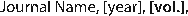
\includegraphics{head_foot/RF}}
\fancyfoot[CE]{\vspace{-7.2pt}\hspace{-14.2cm}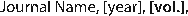
\includegraphics{head_foot/RF}}
\fancyfoot[RO]{\footnotesize{\sffamily{1--\pageref{LastPage} ~\textbar  \hspace{2pt}\thepage}}}
\fancyfoot[LE]{\footnotesize{\sffamily{\thepage~\textbar\hspace{3.45cm} 1--\pageref{LastPage}}}}
\fancyhead{}
\renewcommand{\headrulewidth}{0pt} 
\renewcommand{\footrulewidth}{0pt}
\setlength{\arrayrulewidth}{1pt}
\setlength{\columnsep}{6.5mm}
\setlength\bibsep{1pt}
%%%END OF FOOTER%%%

%%%FIGURE SETUP - please do not change any commands within this section%%%
\makeatletter 
\newlength{\figrulesep} 
\setlength{\figrulesep}{0.5\textfloatsep} 

\newcommand{\topfigrule}{\vspace*{-1pt}% 
\noindent{\color{cream}\rule[-\figrulesep]{\columnwidth}{1.5pt}} }

\newcommand{\botfigrule}{\vspace*{-2pt}% 
\noindent{\color{cream}\rule[\figrulesep]{\columnwidth}{1.5pt}} }

\newcommand{\dblfigrule}{\vspace*{-1pt}% 
\noindent{\color{cream}\rule[-\figrulesep]{\textwidth}{1.5pt}} }

\makeatother
%%%END OF FIGURE SETUP%%%

%%%TITLE, AUTHORS AND ABSTRACT%%%
\twocolumn[
  \begin{@twocolumnfalse}
{
\includegraphics[height=30pt]{head_foot/SM}\hfill\raisebox{0pt}[0pt][0pt]{
\includegraphics[height=55pt]{head_foot/RSC_LOGO_CMYK}}\\[1ex]

\includegraphics[width=18.5cm]{head_foot/header_bar}}\par
\vspace{1em}
\sffamily
\begin{tabular}{m{4.5cm} p{13.5cm} }


\includegraphics{head_foot/DOI} & \noindent\LARGE{\textbf{Instabilities of ring-rivulets: Impact of wettability gradients$^\dag$}} \\%Article title goes here instead of the text "This is the title"
\vspace{0.3cm} & \vspace{0.3cm} \\

 & \noindent\large{Stefan Zitz,\textit{$^{a,b}$} Andrea Scagliarini,\textit{$^{c,d}$} Johan Roenby\textit{$^{a}$}} \\%Author names go here instead of "Full name", etc.

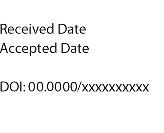
\includegraphics{head_foot/dates} & \noindent\normalsize{
Rivulets and droplets are naturally appearing shapes when small amounts of liquid are brought into contact with a partially wettable substrate.
Here we study, by the means of numerical simulations, the dewetting dynamics of a ring-rivulet deposited on a solid substrate.
First we consider a uniform substrate, similar to the work of Nguyen \textit{et al. Langmuir}, 2012, \textbf{28}, 13960-13967.
We then consider different kinds of surface patterns and show that they not only affect the stability but also the morphology.
Thus making it possible to enhance the probability for a Rayleigh-Plateau type break up into multiple droplets or to accelerate the capillary retraction that stems from the curvature difference of the ring and leads to a single droplet.
}

\end{tabular}

 \end{@twocolumnfalse} \vspace{0.6cm}

]
%%%END OF TITLE, AUTHORS AND ABSTRACT%%%

%%%FONT SETUP - please do not change any commands within this section
\renewcommand*\rmdefault{bch}\normalfont\upshape
\rmfamily
\section*{}
\vspace{-1cm}


%%%FOOTNOTES%%%

\footnotetext{\textit{$^{a}$~IMFUFA, Department of Science and Environment, Roskilde University, Postbox 260, 4000 Roskilde, DK. Tel: +45 2993 1923; E-mail: johan@ruc.dk}}
\footnotetext{\textit{$^{b}$~Research Center Pharmaceutical Engineering GmbH, Inffeldgasse 13, 8010 Graz, Austria, E-mail: stefan.zitz@rcpe.at}}

\footnotetext{\textit{$^{c}$~Institute for Applied Mathematics "M. Picone" (IAC), Consiglio Nazionale delle Ricerche (CNR), Via dei Taurini 19, 00185 Rome, Italy, E-mail: andrea.scagliarini@cnr.it}}
\footnotetext{\textit{$^{d}$~INFN, sezione Roma ``Tor Vergata'', via della Ricerca Scientifica 1, 00133 Rome, Italy}}


%Please use \dag to cite the ESI in the main text of the article.
%If you article does not have ESI please remove the the \dag symbol from the title and the footnotetext below.
\footnotetext{\dag~Electronic Supplementary Information (ESI) available: \href{https://github.com/Zitzeronion/Ring_rivulets}{Ring\_rivulets}. See DOI: 10.1039/cXsm00000x/}
%additional addresses can be cited as above using the lower-case letters, c, d, e... If all authors are from the same address, no letter is required

%\footnotetext{\ddag~Additional footnotes to the title and authors can be included \textit{e.g.}\ `Present address:' or `These authors contributed equally to this work' as above using the symbols: \ddag, \textsection, and \P. Please place the appropriate symbol next to the author's name and include a \texttt{\textbackslash footnotetext} entry in the the correct place in the list.}


%%%END OF FOOTNOTES%%%

%%%MAIN TEXT%%%%
\section{Introduction}
\label{sec:intro}
Thin liquid films and droplet are widespread in our every day life and play a crucial role
in a host of natural and technological applications, from painting and coating to lab-on-a-chip devices to biofluidics~\cite{degennesCapillarityWettingPhenomena2004, ronsinPhaseFieldSimulationsMorphology2022,fockeLabonaFoilMicrofluidicsThin2010}.
Understanding their dynamics and controlling their stability is, therefore, a central problem for applied research in process engineering and nanotechnology~\cite{singhInkjetPrintingProcess2010, quereFluidCoatingFiber1999, utadaDrippingJettingDrops2007}, but also poses fundamental questions lying at the crossroads between fluid dynamics and chemical physics~\cite{oronLongscaleEvolutionThin1997, beckerComplexDewettingScenarios2003, thielePatternedDepositionMoving2014, wilczekSlidingDropsEnsemble2017, peschkaSignaturesSlipDewetting2019}.
Dewetting induced by intrinsic instabilities of the film and/or impurities on 
the substrate surface, for instance, can undermine the effectiveness of a coating process
~\cite{bonnWettingSpreading2009, chenWrinklingInstabilitiesPolymer2012}. 
On the other hand, breakup of deposited structures such as rivulets is exploited
in the generation of droplets {\it on demand}~\cite{}.
All these phenomena involve inherently multiscale problems, that span from the molecular motion at the three phase contact line to the nano-/mircoscale thickness of the film up to the macroscopic area the coating covers, thus posing not trivial computational challenges.

A thin film model can also be used to study the dynamics of ring-rivulet on a solid substrate.
This particular fluid structure has been point of interest to previous studies~\cite{nguyenCompetitionCollapseBreakup2012, gonzalezStabilityLiquidRing2013, wuCompetingLiquidPhase2011, edwardsControllingBreakupToroidal2021} and differs considerably from a straight liquid rivulet~\cite{diezBreakupFluidRivulets2009, diezStabilityFinitelengthRivulet2009, diezInstabilityTransverseLiquid2012} due to the introduction of multiple unbalanced curvatures.
Recently, Suo et al.~\cite{suoDewettingCornerFilm2023} have studied a related problem where the film admits a wedge shape and a solid cylinder fills the inner part of the ring. 
The ring is therefore not allowed to contract, but can breakup and form droplets.
They further show a good agreement between theory and simulations as well as a clear dependence of the dynamics on the initial width of the film and the contact angles at each boundary.
Self- and direct assembly of nanomaterials from liquid nanostructures has been one of the driving forces for the study of Nguyen et al.~\cite{nguyenCompetitionCollapseBreakup2012} and earlier studies of Wu et al.~\cite{wuBreakupPatternedNanoscale2010} where they showed that liquid-metal rings are suited to form arrays of droplets.
Diez et al.~\cite{diezBreakupFluidRivulets2009, diezStabilityFinitelengthRivulet2009} laid the theoretical foundation for a straight rivulet in their work using linear stability analysis (LSA) and numerical simulations. 
Later, Gonz{\'a}lez et al.~\cite{gonzalezStabilityLiquidRing2013} extend these results towards a cut torus shape and called it liquid ring, making it therefore possible to predict wavelengths for the most unstable mode and describing the competing time scales for collapse and breakup.
In their study they however point out that for thin films, where the disjoining pressure~\cite{schwartzSimulationDropletMotion1998, beckerComplexDewettingScenarios2003, oronLongscaleEvolutionThin1997} can not be ignored, e.g. a few nanometres in thickness, the LSA overpredicts  the expected number of droplets after breakup.
While the disjoining pressure model seems to choose a larger wavelength before breakup Nguyen et al.~\cite{nguyenCompetitionCollapseBreakup2012} showed that molecular dynamics (MD) simulations seem to agree with the LSA when it comes to the number of droplets.
About a decade later Edwards et al. studied liquid rings with numerical and experimental tools~\cite{edwardsControllingBreakupToroidal2021}.
They considered contact angles beyond the long wave approximation ($\theta > 1$) and electrowetting~\cite{mugeleElectrowettingConvenientWay2005}. 
In their work they showed that different electric potentials can be used not only to control the number of droplets after breakup but also to fully reverse the process.
Beside the work on thin films Mehrabian and Feng~\cite{mehrabianCapillaryBreakupLiquid2013} showed simulations and experiments of a freely suspend liquid torus in another fluid.
In their study they found that the time to breakup depends inversely on the amplitude of the initial perturbation and the initial thickness of the torus.
They further discuss the influence of the viscosity contrast between the liquids, as this difference has an effect both on the capillary waves and the retraction velocities.
 

We are going to address the thin ring-rivulet problem with a further complication, namely the introduction of a wettability gradient.
With recent developments in surface chemistry and the emerging technology of switchable substrates~\cite{xinReversiblySwitchableWettability2010, stuartEmergingApplicationsStimuliresponsive2010,chenThermalresponsiveHydrogelSurface2010, ichimuraLightDrivenMotionLiquids2000, mugeleElectrowettingConvenientWay2005, edwardsControllingBreakupToroidal2021} local precise wettability gradients are more attainable than ever..
It has been shown numerous times that wettability gradients are able to transport droplets, see Ref.~\cite{liuActuatingWaterDroplets2015} or more recently with time dependent patterns Refs.~\cite{grawitterSteeringDropletsSubstrates2021, zitzControllingDewettingMorphologies2023}, thus having a wettability gradient should allow for a more fine grained the control of the intermediate ring-rivulet states.
To this end, we show that it is possible to steer the number of droplets after breakup and furthermore be even able to set the spacing between neighboring droplets.
That said, the inverse can also be achieved, thus initial conditions that lead to breakup into multiple droplets can be steered to collapse into a single droplet. 
Having arbitrary control over these quantities will in fact make this process more applicable for the production of nanomaterials. 

The outline of the paper is as follows: In the next section, Sec.~\ref{sec:method} we introduce the method we use to run numerical experiments.
We then present our results in Sec.~\ref{sec:dynamics}, starting with a comparison with the literature and then present the impact of the wettability gradient.
In the last section, Sec.~\ref{sec:conclu} we give a short summary, highlighting important results and conclude with an outlook of possible research applications.

\section{Simulation method}
\label{sec:method}
For the time resolved simulations of a thin liquid ring-rivulet we use a recently developed lattice Boltzmann method (LBM)~\cite{zitzLatticeBoltzmannMethod2019, zitzLatticeBoltzmannSimulations2021, zitzSwalbeJlLattice2022, zitzControllingDewettingMorphologies2023}. 
This method is an effective numerical scheme to solve the thin film equation (TFE),  
\begin{equation}\label{eq:thinsolve}
     \partial_t h(\mathbf{x},t) = \nabla\cdot\left(M_{\delta}(h)\nabla p\right),
\end{equation}
where $\mathbf{x} = (x,y)$ and $\nabla = (\partial_x, \partial_y)$.
The mobility function $M_{\delta}(h) = \frac{h^2}{\mu\alpha_{\delta}(h)}$ with 
\begin{equation}\label{eq:alphafric}
    \alpha_{\delta}(h) = \frac{6h}{(2 h^2 + 6 \delta h + 3 \delta^2)},
\end{equation}
which for the no-slip boundary condition $(\delta \rightarrow 0)$ becomes $M_{0}(h) = h^3/3\mu$, where $\delta$ is an effective slip length and $\mu$ is the dynamic viscosity, both values can be found in App.~\ref{app:numerics}.
We like to point out, however, that the slip length value is within the weak/intermediate slip regime~\cite{peschkaSignaturesSlipDewetting2019,fetzerQuantifyingHydrodynamicSlip2007, munchLubricationModelsSmall2005} and has been used in previous work~\cite{zitzControllingDewettingMorphologies2023}.
The pressure $p$ in Eq.~(\ref{eq:thinsolve}) is given by,
\begin{equation}\label{eq:filmpressure}
    p = - \gamma\nabla^2 h -\Pi(h),
\end{equation}
with $\Delta h$ being the 2D Laplacian of the liquid-gas interface and $\Pi(h)$ is a so-called disjoining pressure~\cite{schwartzSimulationDropletMotion1998, crasterDynamicsStabilityThin2009, nguyenCompetitionCollapseBreakup2012, gonzalezStabilityLiquidRing2013}
\begin{equation}\label{eq:disjoinpressure}
    \Pi(h,\theta) = \frac{2\gamma}{h_{\ast}}[1-\cos\theta(\mathbf{x})]\left[\left(\frac{h_*}{h}\right)^3 -\left(\frac{h_*}{h}\right)^2\right],
\end{equation}
where $\gamma$ is the surface tension, $h_{\ast}$ is a precursor thickness, see App.~\ref{app:numerics}, at which $\Pi(h_{\ast}, \theta) = 0$ and $\theta$ is an equilibrium contact angle.
By varying $\theta$ in Eq.~(\ref{eq:disjoinpressure}) we have an effective model for a patterned substrate, see e.g., Refs~\cite{zitzLatticeBoltzmannSimulations2021, zitzControllingDewettingMorphologies2023}. 
The contact angle, in agreement with the lubrication approximation~\cite{oronLongscaleEvolutionThin1997, crasterDynamicsStabilityThin2009}, is set within the bounds $[\pi/18, 2\pi/9]$, except for the banded pattern, see Sec.~\ref{subsubsec:banded}. 

Our strategy is therefore to iterate Eq.~(\ref{eq:thinsolve}) in time and let the rivulet find a stable configuration, with some upper limit on simulation time as discussed in App.~\ref{app:numerics}.
This stable configuration can either be several disconnected droplets if the rivulet breaks up or a single coalleased droplet in the middle of the domain.  

\subsection{Initial conditions}
\begin{figure}
\centering
  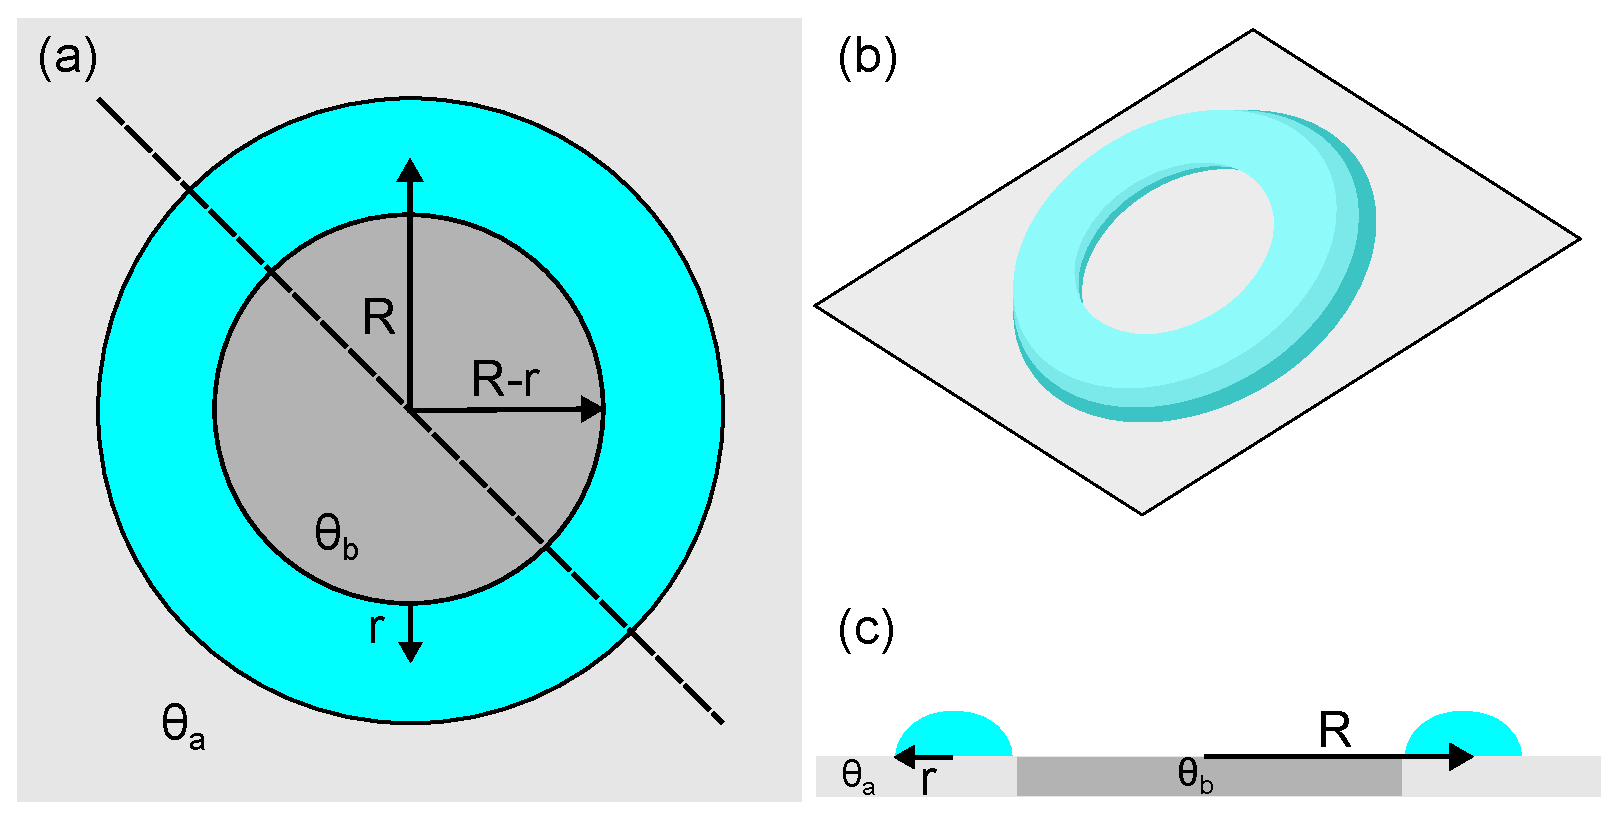
\includegraphics[width=0.45\textwidth]{ringrivulet_shema}
  \caption{Schematic setup of our initial conditions. In (a) we show the top view where $R$ and $r$ are the two different radii and $\theta_a$ and $\theta_b$ can be different contact angles. 
  In (b) we show an isometric view of the initial condition.
  By cutting along the dashed line in (a) we get the side view of (c).}
  \label{fig:ringschema}
\end{figure}

The initial thickness profile $h(\mathbf{x}, t=0)$ of the film is set by an implicit equation for a torus with radial symmetry along the z-axis according to
\begin{equation}\label{eq:torus}
    h(\mathbf{x}, t=0) = \sqrt{r_0^2 - \left(R_0-\xi\right)^2} - r_0\cos(\theta) + \varepsilon(\mathbf{x})\mathcal{N},
\end{equation}
where $\xi = \sqrt{(x-x_0)^2+(y-y_0)^2}$ is a radial coordinate, $R_0$ is the major radius and $r_0$ is the minor radius of the torus.
The center of the torus is at $(x_0,y_0)$ and for all numerical experiments set to the center of the numerical domain.
Eq.~(\ref{eq:torus}) allows for negative thickness values, however, we only consider the upper half of the torus as shown in Fig.~\ref{fig:ringschema}. 
The second term in Eq.~(\ref{eq:torus}) is to cut the upper half to a smaller contact angle.
The third term adds white noise to the initial condition, $\mathcal{N}$ is a gaussian with zero mean and $\varepsilon(\mathbf{x})$ is an amplitude that is 
\begin{equation}
    \varepsilon(\mathbf{x}) =
    \begin{cases}
        10^{-2}\quad \textbf{if}~h(\mathbf{x}) > h_{\ast}\\
        0~~\quad\quad \textbf{else}
    \end{cases}
    .
\end{equation} 
We further require that any $h(\mathbf{x}) < 0$ is set to $h_{\ast}$.
The lubrication approximation does in fact not allow us to use the initial conditions in Refs.~\cite{nguyenCompetitionCollapseBreakup2012, wuBreakupPatternedNanoscale2010} or use contact angles as large as in Edwards et al.~\cite{edwardsControllingBreakupToroidal2021} but are in agreement with Gonz{\'a}lez et al.~\cite{gonzalezStabilityLiquidRing2013}.

Our main interest is focused on the impact of a pattern on the evolution of the ring-rivulet. 
As indicated with two $\theta$ values in Fig.~\ref{fig:ringschema} we use different wettability patterns.
A natural starting point that allows to compare to Refs.~\cite{gonzalezStabilityLiquidRing2013, nguyenCompetitionCollapseBreakup2012, wuBreakupPatternedNanoscale2010} is $\theta(\xi) = \theta_0$,where $\theta_0$ is a constant.
In the second scenario we consider a banded case which is somewhat related to the work of Edwards et al.~\cite{edwardsControllingBreakupToroidal2021}. 
Here the ring-rivulet has the same contact angle as its immediate surrounding and the rest of the substrate has a higher contact angle
\begin{equation}\label{eq:theta_band}
    \theta(\xi) =\begin{cases}
        \theta_a,\quad \text{if}~h(\xi\pm \delta\xi) > 0\\
        \theta_b,\quad \text{else}
    \end{cases}.
\end{equation}
The addition of $\delta\xi$ widens the band and allow the ring-rivulet to contract a bit.  
Lastly, we consider a linear radial wettability gradient towards the middle
\begin{equation}\label{eq:theta_grad}
    \theta(\xi) = \frac{\theta_{a}-\theta_{b}}{R_0} \xi + \theta_{b},
\end{equation}
where $\theta_{a}\neq\theta_{b}$.
We consider both possibilities, thus a negative wettability gradient ($\theta_a > \theta_b$) and a positive wettability gradient ($\theta_a < \theta_b$).

These three expressions for $\theta$ are then used in Eq.~(\ref{eq:disjoinpressure}) which is part of the pressure calculation in Eq.~(\ref{eq:thinsolve}).
The numerical experiments therefore create a dynamic response of the initial condition Eq.~(\ref{eq:torus}) to each pattern.

\section{Dynamics of a ring-rivulet}
\label{sec:dynamics}
\begin{figure*}
    \centering
    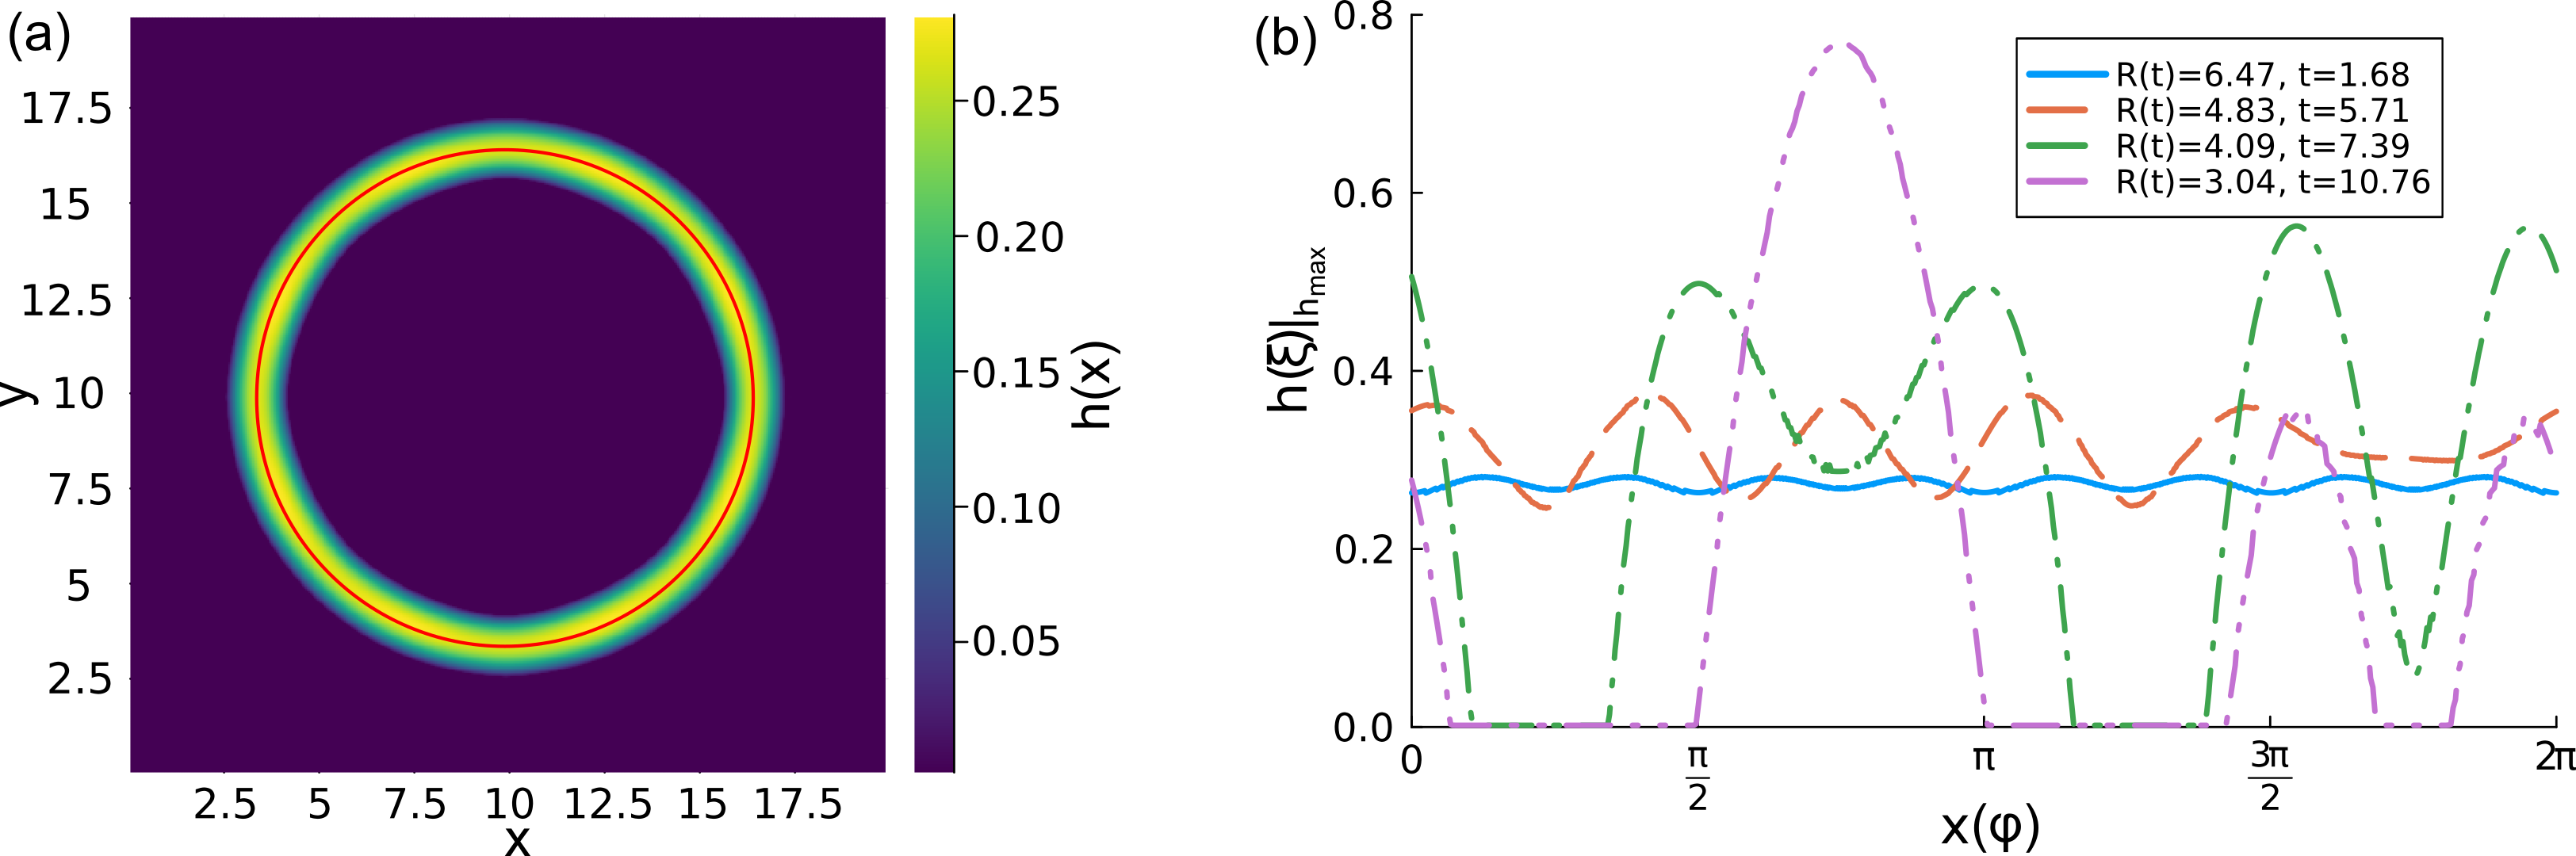
\includegraphics[width=0.95\textwidth]{assets/heatcirc.png}
    \caption{(a) Heatmap of the film thickness at $t=1.68\tau_m$ for $\psi_0 = 0.21$. 
    All length scales are normalized by $H_D = 25.67$. 
    The red ring in the middle of the rivulet is depicted as blue line plot in (b).
    In (b) we show circular cuts normalized to $2\pi$, shown in different colors and line styles, for different time steps normalized by Eq.~(\ref{eq:tau_m}) at $\xi(h_{\max})$.
    The ring-rivulet initially chooses a breakup mode that lead to eight droplets, however with time it breaks into three distinct droplets, indicated by the three maxima of the purple curve.}
    \label{fig:ThreeDToOneD}
\end{figure*}
The time resolved dynamics of initial fluid structures Eq.~(\ref{eq:torus}) are surprisingly rich, with one case outlined in Fig.~\ref{fig:ThreeDToOneD}.
It has been shown in several studies that the torus geometry is an unstable fluid state~\cite{gonzalezStabilityLiquidRing2013, mehrabianCapillaryBreakupLiquid2013, edwardsControllingBreakupToroidal2021, wuBreakupPatternedNanoscale2010} which is prone to Rayleigh-Plateau and other contact line instabilities. 
The fluid interface itself admits three distinct curvatures, two horizontal ones at the two triple lines between substrate fluid and gas, $\kappa_a = 1/(R+r)$ and $\kappa_b = 1/(R-r)$ as indicated in Fig.~\ref{fig:ringschema}, and one vertical along the liquid-gas interface $\kappa_r = 1/r$.
We remark that both $R$ and $r$ are time-dependent quantities that change as the rivulet evolves.
At $t=0$ we have $R_0 = R$ and $r = r_0\sin(\theta)$, thus $r_0$ is the radius of the circle from which the rivulet is cut and at $\theta = \pi/2$ we have $r=r_0$, see Eq.~(\ref{eq:torus}).
These curvatures lead to capillary forces and small instabilities can quickly be amplified and destabilize a torus~\cite{mehrabianCapillaryBreakupLiquid2013} or a liquid ring~\cite{gonzalezStabilityLiquidRing2013}. 
The result can either be a single droplet due to contraction, which is also referred to as collapse or multiple small droplets due to breakup.
Within our numerical experiments we indeed observe both scenarios.

\subsection{Stability and time scales}\label{subsec:stability}
Among the dynamical properties that this system admits we first like to address the stability of the ring-rivulet and the associated time scales.
In previous studies~\cite{gonzalezStabilityLiquidRing2013} the focus was set on the three-phase contact lines and the LSA predictions agreed well with the slip model simulations.
Among the many results of this work is the fact that the varicos modes are always growing stronger than the zigzag modes.
The stability, then, is associated with the width of the ring-rivulet $w = 2r$ as well as the ratio of radii $\psi_0 = 2r/R_0 = w/R_0$.
When the width approaches zero, $w \rightarrow 0$, the rivulet breaks up and is likely to form independent droplets.

We use a slightly different measure to access the stability of the rivulet. 
Instead of directly working with the three-dimensional data we take a circular cut (red circle in Fig.~\ref{fig:ThreeDToOneD}(a)) along the rivulet and measure
\begin{equation}\label{eq:delta-h-measure}
    \Delta h = (h_{\max} - h_{\min})_{\xi = \xi(h_{\max})},
\end{equation}
which can be computed from Fig.~\ref{fig:ThreeDToOneD}(b).
This measure has the advantage that it is well within the rivulet and thus should filter out a constant background from the precursor film $h_{\ast}$, see Eq.~(\ref{eq:disjoinpressure}).

\begin{figure}
    \centering
    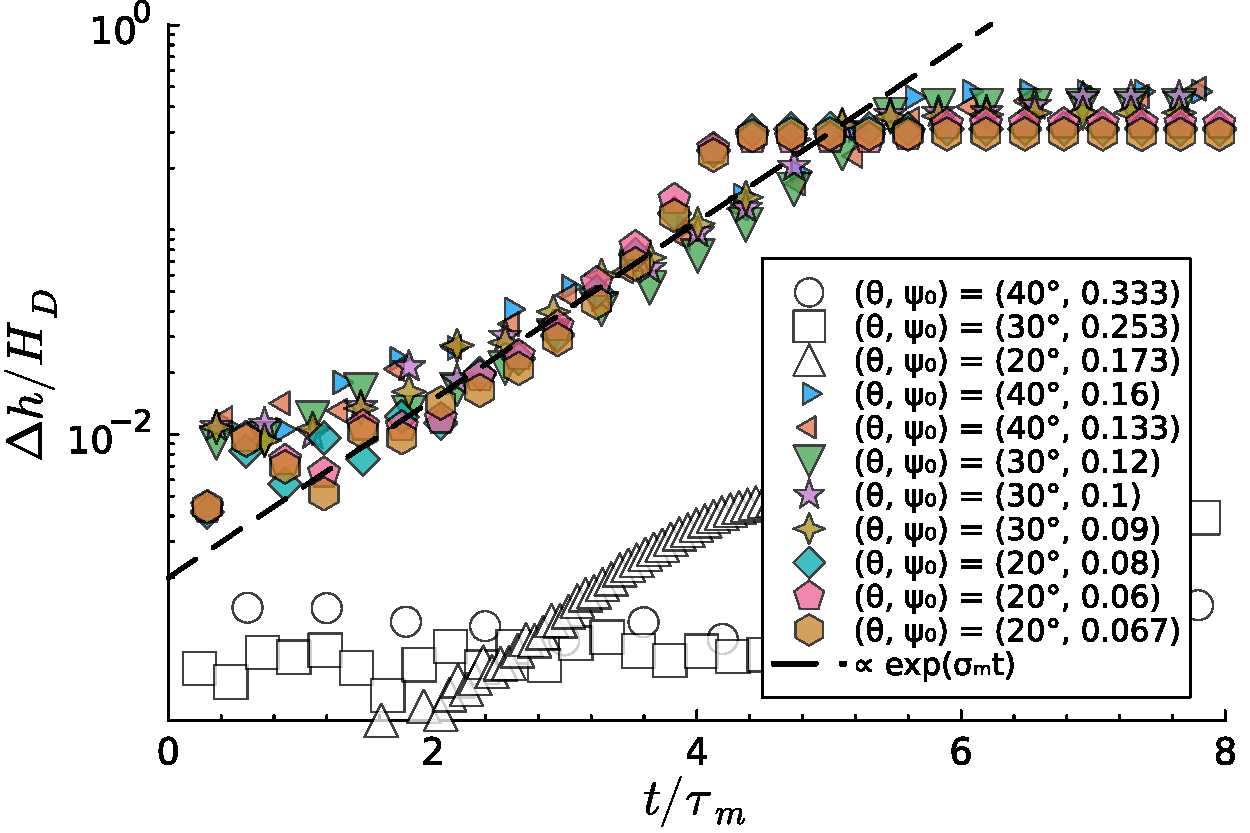
\includegraphics[width=0.45\textwidth]{assets/growth-breakup.pdf}
    \caption{Thickness difference $\Delta h$ normalized by the height of a spherical cap droplet that contains all liquid $H_D$ along the curve at radius $\xi(h_{\max})$ over time normalized by $\tau_{m}$~\cite{wuBreakupPatternedNanoscale2010} for the uniform pattern. 
    Different symbols depict different initial conditions. 
    Full or empty symbols distinguish between breakup and collapse. 
    The black dashed curve shows an exponential growth $e^{\sigma_m t}$, see Eq.~(\ref{eq:growth-sigma}).
    }
    \label{fig:first_growth}
\end{figure}
As a criterion for a break up using a circular cut we assume $\Delta h \approx 2\max{h(\mathbf{x},0)}$. 
In previous studies, it has been shown that the break up follows and exponential growth~\cite{wuBreakupPatternedNanoscale2010, gonzalezStabilityLiquidRing2013, nguyenCompetitionCollapseBreakup2012}.
% TODO: Needs to be explained better and worked out why it fits so well!
To address this statement we use the growth rate $\sigma_m$ which reads
\begin{equation}\label{eq:growth-sigma}
    \sigma_m = \frac{\gamma a \theta^{3/2}\sqrt{\theta - \sin(2\theta)/2}}{6\mu\sin(\theta)\sqrt{A}}, 
\end{equation}
where $a$ is a numerical constant which is set to $a = 0.0379$ according to Ref.~\cite{wuBreakupPatternedNanoscale2010, diezBreakupFluidRivulets2009} and $A$ is half of the area of the cross-section of the rivulet as shown in Fig.~\ref{fig:ringschema}(c).
We like to mention that Eq.~(\ref{eq:growth-sigma}) differs from ref~\cite{wuBreakupPatternedNanoscale2010} by a factor of $\theta^{-3/2}$, however using $\sigma_m$ we can derive a timescale $\tau_m$ by simply inverting the growth rate  
\begin{equation}\label{eq:tau_m}
    \tau_{m} = \frac{1}{\sigma_m} = \frac{6\mu\sin(\theta)\sqrt{A}}{\gamma a \theta^{3/2}\sqrt{\theta - \sin(2\theta)/2}}.      
\end{equation}
In Fig.~\ref{fig:first_growth} we show $\Delta h$ data at different time steps for the uniform pattern normalized by their respective $H_D$ and $\tau_m$ as the different symbols.  
We find a reasonable collapse for the full symbols with this rescaling and as a guide to eye we add a black dashed line that is proportional to $e^{\sigma_m t}$, see Eq.~(\ref{eq:growth-sigma}). 
The empty symbols on the other hand do not show a pronounced growth, with the one exception of the open triangles ($\triangle$, $\psi_0 = 0.173$). 
The filled symbols are numerical experiments that lead to break up of the rivulet, while the empty symbols display the collapse into a single droplet.

Therefore, the $\Delta h$ values along $\xi(h_{\max})$ of the rivulet allow us to distinguish between initial conditions that lead to breakups and droplet fragmentation, as such following the dashed line in Fig.~\ref{fig:first_growth}, and a collapse into a single droplet as shown by the open symbols in Fig.~\ref{fig:first_growth}.
The open triangles ($\triangle$, $\psi_0 = 0.173$) actually mark an edge case in which $\Delta h$ grows with a similar slope as the filled symbols, however the timescale on which the instability grows is too long as compared to the collapse timescale. 
We will get back to this point in Sec.~\ref{subsec:wettability} where we discuss the banded case, Eq.~(\ref{eq:theta_band}) and show that the collapse is fast for larger $\psi_0$s as compared to the breakup instability.

\subsection{Breakup modes and droplets}\label{subsec:drop-counting}
\begin{figure}
    \centering
    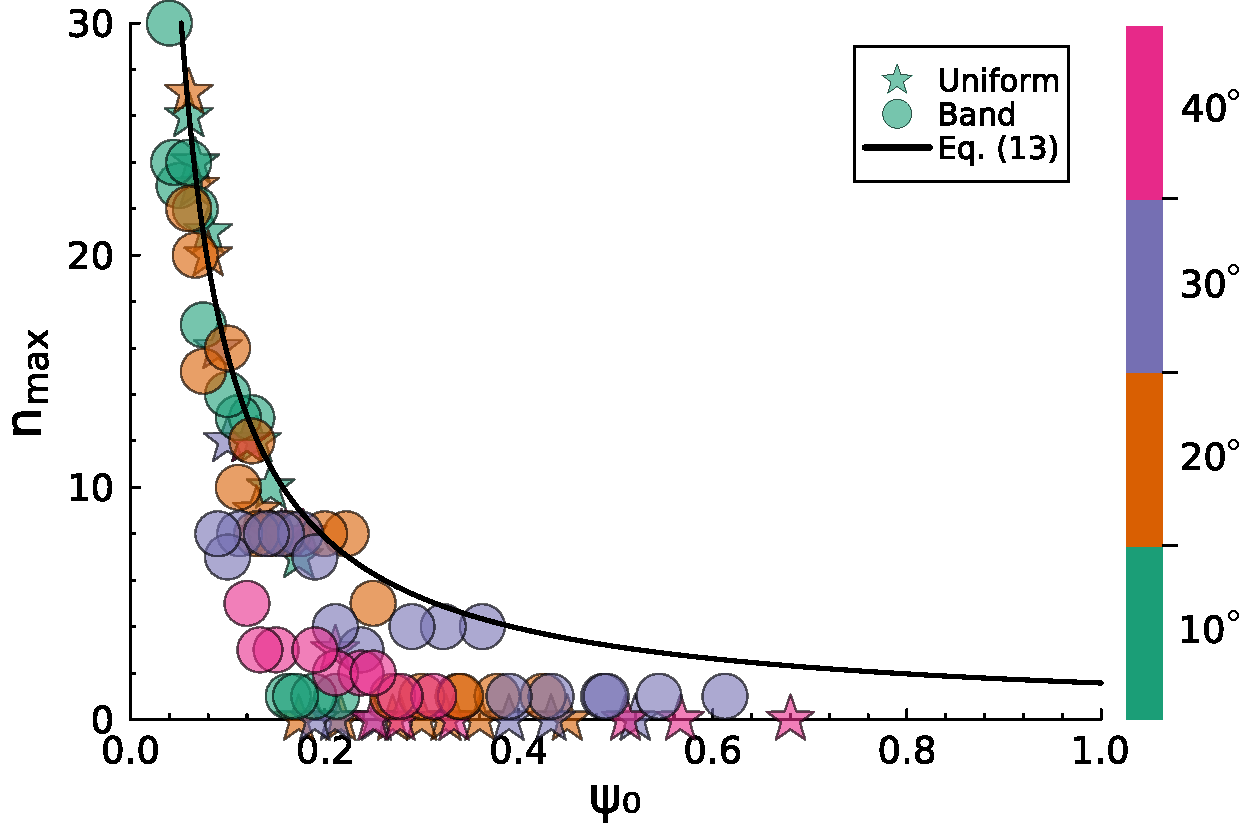
\includegraphics[width=0.45\textwidth]{assets/maxdropsUniBandCC.pdf}
    \caption{Number of maximal droplets $n_{max}$ over reduced aspect ratio $\psi_0$.
    Different symbols show different substrates, where the uniform substrate is shown by blue bullets (\textcolor{black}{$\bullet$}) and Eq.~(\ref{eq:theta_band}) by orange stars (\textcolor{black}{$\star$}).
    We compare our results to the linear stability analysis (LSA) from Gonz{\'a}lez et al.~\cite{gonzalezStabilityLiquidRing2013}}
    \label{fig:max_drops}
\end{figure}

Given the initial conditions of the ring-rivulet can we predict if there is a collapse or a breakup? 
Can we further predict in the case of breakup how many droplets are formed?
While this may sound like a funny question it bares great impact for nanostructuring and/or self-assembly, thus having predictive power is of great interest.
Both questions were addressed by Gonz{\'a}lez et al.~\cite{gonzalezStabilityLiquidRing2013}. 
The maximal number of droplets $n_{\max}$ can be computed with a complex system of equations which are based on the most unstable mode.
They furthermore found a surprisingly good approximation that can be calculated from initial conditions, 
\begin{equation}\label{eq:maxDrops}
    n_{\max, app} = \frac{\pi}{2\psi_0}.
\end{equation}
Therefore, it seems as if the number of droplets is simply set at $t=0$ by geometry of the rivulet.
This result has been tested and shown to agree well with MD simulations by Nguyen et al.~\cite{nguyenCompetitionCollapseBreakup2012}. 

However, Gonz{\'a}lez et al.~\cite{gonzalezStabilityLiquidRing2013} pointed out that the LSA and thus $n_{\max}$ fall short if one considers a disjoining pressure model, see Eq.~(\ref{eq:disjoinpressure}).
They report that although initially the rivulet adapts to its most unstable mode it does not necessary break up into $n_{\max}$ droplets, especially for $\psi_0 > 0.15$. 
They also point towards the experiments of Wu et al.~\cite{wuCompetingLiquidPhase2011} where a similar mismatch with theoretical predictions was observed.

We perform a similar analysis and count the number of droplets during our numerical experiments and adopted the scheme introduced by Gonz{\'a}lez et al.~\cite{gonzalezStabilityLiquidRing2013}, thus count the collapse as zero droplets, one off center droplet as one, two droplets as two and so on.
The result is shown in Fig.~\ref{fig:max_drops}, where the black line is given by Eq.~(\ref{eq:maxDrops}) and the different symbols refer to a uniform substrate and the band pattern Eq.~(\ref{eq:theta_band}).
% Our results tend to agree with the observations made by Gonz{\'a}lez et al.~\cite{gonzalezStabilityLiquidRing2013}.
In Fig.~\ref{fig:ThreeDToOneD} we actually observe a transition from $n = 8$ (blue curve) to $n = 3$ (purple curve), observing only three droplets after breakup.

% We can further quantify this behavior in terms of time scales for both the collapse and the breakup of the ring-rivulet.
In Fig.~\ref{fig:max_drops} we see that for larger $\psi_0$-values theory and our numerical experiments do not match.
In fact, for $\psi_0 > 0.22$ the ring-rivulet on the homogeneous substrate (\textcolor{jlorange}{$\star$}) favours the collapse $n = 0$. 
It is therefore fair to assumes that the growth-rate of the instability is slower than the rate of collapse, thus $t_b > t_c$ for $\psi_0 > 0.22$, see Fig.~\ref{fig:first_growth} empty symbols.
In Fig.~\ref{fig:timescaleDifference} we measured these time scales as function of $\psi_0$ and normalized them with their respective $\tau_m$, Eq.~(\ref{eq:tau_m}).
\begin{figure}
    \centering
    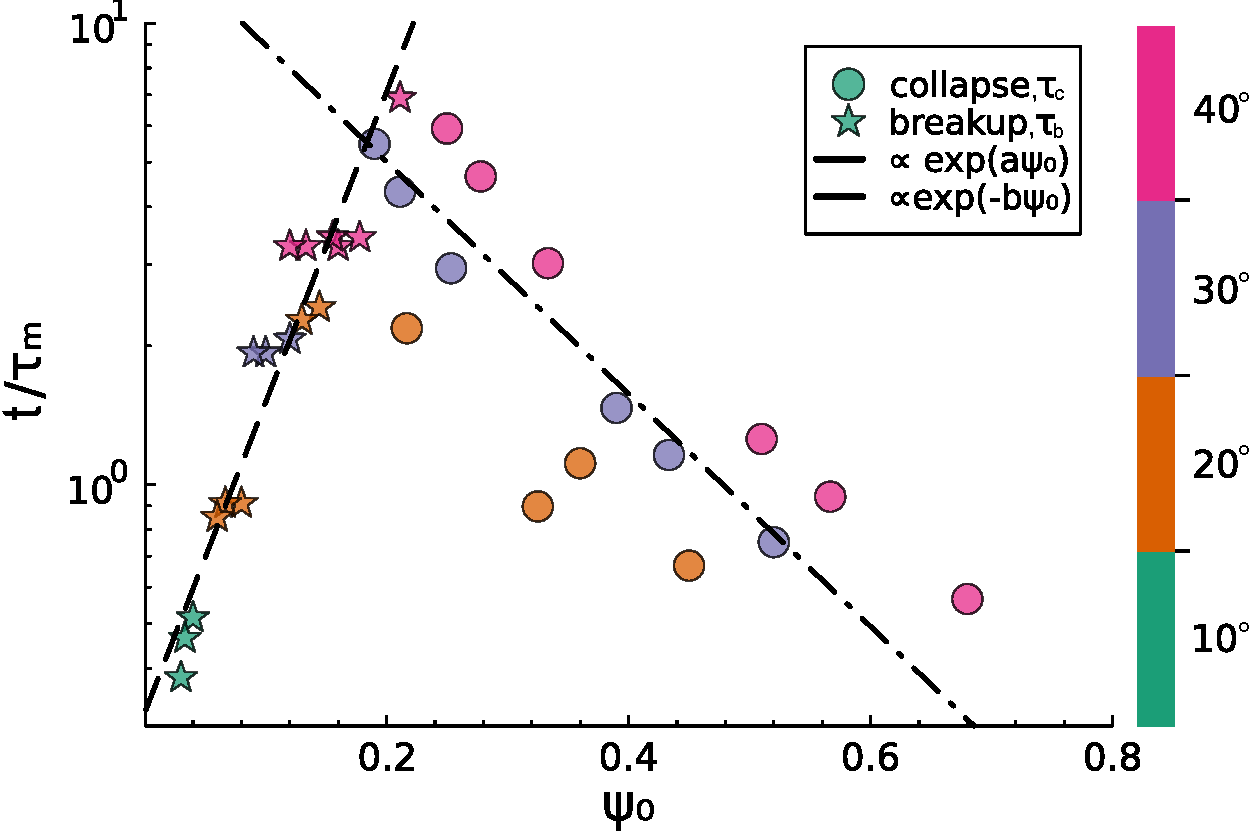
\includegraphics[width = 0.45\textwidth]{assets/uniform_timescalesCC.pdf}
    \caption{Breakup and collapse times $\tau$ for all numerical experiments on a uniform substrate.
        On the x-axis we use the dimensionless length scale $\psi_0$ and the y-axis displays either the breakup- or collapse time $\tau$ with stars (\textcolor{jlorange}{$\star$}) or bullets (\textcolor{jlblue}{$\bullet$}) respectively.
        The dashed line serves as a guide to eye and shows an exponential growth that is in agreement with the breakup data. 
        The dash-dotted line shows and exponential decay which can be motivated by the collapse data.
        % We do not observe breakup events for ring-rivulets with $\psi_0 > 0.22$. 
        }
    \label{fig:timescaleDifference}
\end{figure}
First, the data suggest that there is no clear boundary that distinguishes between collapse and breakup.
We find a region around $\psi_0 \approx 0.2$ where the collapse times and the breakup times are of similar magnitude.
For smaller $\psi_0$, the rivulets are more likely to break up into multiple droplet, while for larger $\psi_0$ the collapse is the more likely outcome of a numerical experiment.

\subsection{Wettability patterns}\label{subsec:wettability}
In the previous sections we focused on the role of curvatures and thus used $\psi_0$ indifferent of the wettability. 
The concrete initial condition and thus $\psi_0$ is however a function of $\theta$, see Eq.~(\ref{eq:torus}).
A lower contact angle yields a smaller rivulet, both in height and width for the same $r_0$ value.
Fig.~\ref{fig:first_growth} shows that upon rescaling time with Eq.~(\ref{eq:tau_m}), which is a function of $\theta$, the breakup data collapses and follows the predicted $\sigma$ line.
We also saw that Eq.~(\ref{eq:maxDrops}) holds true for $\psi_0 \leq 0.25$, for larger $\psi_0$ values the collapse is the more likely outcome on a uniform substrate.

In order to further investigate the ring-rivulet we now make the contact angle a function of space, thus using an effective model of a patterned substrate. 
Small amounts of liquids on patterned substrates have been studied extensively, see for example Refs.~\cite{savvaDropletMotionInclined2013, vellingiriDropletSpreadingChemically2011, wangWettingEffectPatterned2023, wuInvestigationEquilibriumDroplet2019} to name but a few.
We discuss two types of patterns, where the first one serves as an effective boundary which removes the collapse mode and the second one helps us to understand the force balance between wetting and retraction of the ring-rivulet, see Eqs.~(\ref{eq:theta_band}-\ref{eq:theta_grad}).

\subsubsection{Banded pattern}\label{subsubsec:banded}
The first pattern Eq.~(\ref{eq:theta_band}) constrains the ring-rivulet to its initial area with some additional margin $\delta\xi$.
This is realized by using $\theta_a \in [10^{\circ}, 20^{\circ}, 30^{\circ}, 40^{\circ}]$ and $\theta_b = 60^{\circ}$, which yields a contact angle contrast $\Delta\theta \in [50^{\circ}, 40^{\circ}, 30^{\circ}, 20^{\circ}]$.
While this choice seem to contracting the long wave approximation, we actually do not see the film penetrating the $\theta_b$ region in our numerical experiments.
Thus, the substrate area $\pm\delta\xi$ away from the ring-rivulets base can be understood as an effective barrier. 
Edwards et al.~\cite{edwardsControllingBreakupToroidal2021} performed related experiments where they were able to remove the coalescence mode with elaborate surface coatings and used electrowetting to dynamically modify the contact angle.

\begin{figure}
    \centering
    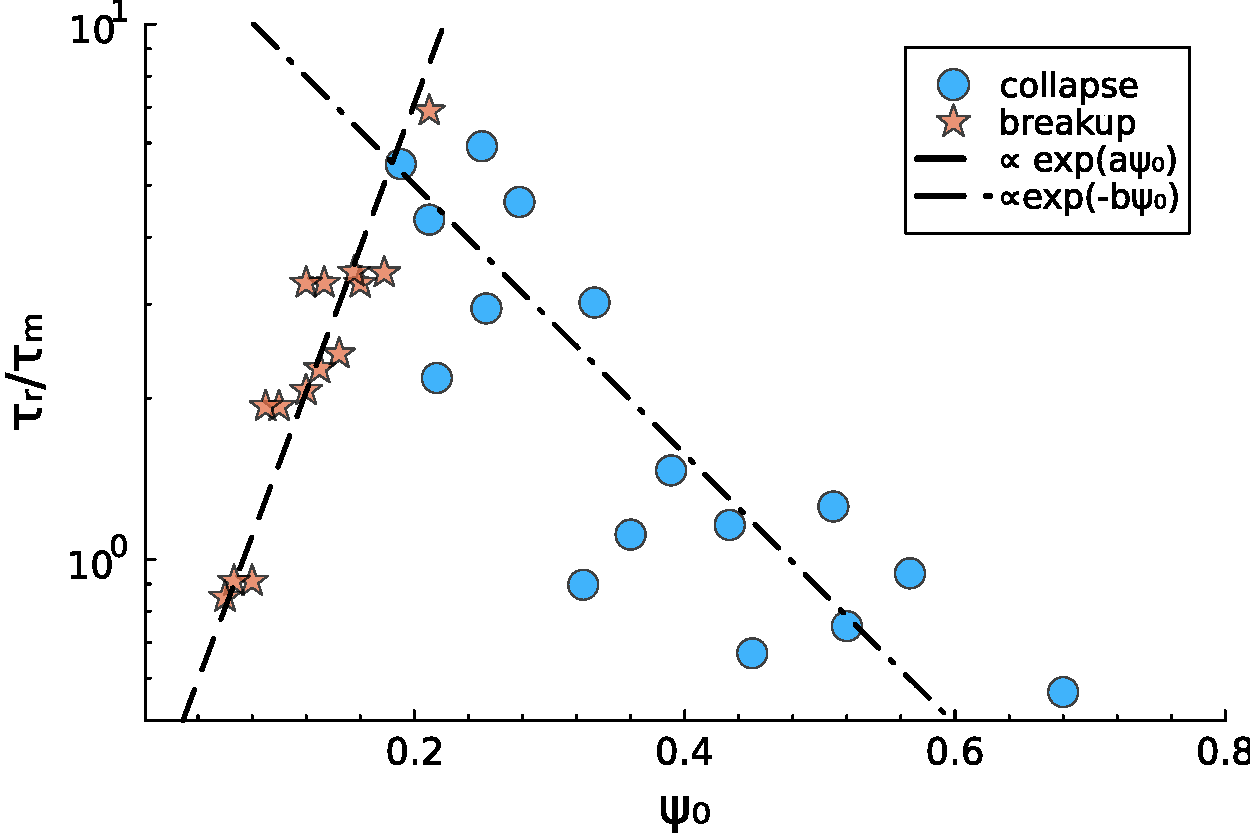
\includegraphics[width=0.48\textwidth]{assets/bandBreakup_timescales.pdf}
    \caption{Breakup times $\tau_b$ normalized by their respective $\tau_m$ for the banded case Eq.~\ref{eq:theta_band}.
    Different colors depict different contact angle contrasts $\Delta\theta$.
    The dashed line is a linear function of $\psi_0$. %with $La = \gamma\rho R_0/\mu^2$ as slope.
    }
    \label{fig:bandBreakupT}
\end{figure}
Because the initial configuration is unstable, the ring-rivulet will eventually rupture and form droplets, this however can be on long time scales depending on $\psi_0$.
In Fig.~\ref{fig:bandBreakupT} we measure the rupture times $\tau_b$ normalized by their respective $\tau_m$ for different initial conditions on the banded substrate.
Different colors indicate different contact angle contrasts $\Delta\theta$ and although there is not a complete collapse of the data, it seems that there is a linear trend between $\tau_b/\tau_m$ and $\psi_0$.
To highlight this statement we add a linear fit in Fig.~\ref{fig:bandBreakupT} as a black dashed line. 

Although having numerical experiments run up to $t = 25\tau_m$ we do not always observe the breakup. 
This is indicated in by the $n_{\max} = 1$ data in Fig.~\ref{fig:max_drops}, where the bullets (\textcolor{black}{$\bullet$}) show data from the banded pattern. 
In those simulations the ring-rivulet has not ruptured at the end of the simulation time.
However, $\Delta h$ measurements show growth in some cases.
% In contrast to the uniform substrate we do not see any $n_{\max} = 0$ event. 
We see that the predicted number of droplets Eq.~(\ref{eq:maxDrops}) does not fit the data as good as for the uniform substrate. 
Similarly to the uniform substrate and in agreement with previous work~\cite{gonzalezStabilityLiquidRing2013} we see similar behavior as in Fig.~\ref{fig:ThreeDToOneD}.
Thus, having $n = n_{\max}$ for early time scales but at rupture we get $n < n_{\max}$.

\subsubsection{Linear wettability gradients}\label{subsubsec:linwettgrad}
So far we have shown that our numerical experiments can, first, reproduce known results and second are able to address the aspect of wettability.
We find that a larger contact angle leads to deviations from Eq.~(\ref{eq:maxDrops}) but growthrates $\sigma_m$ can be collapsed.
Further we have shown that a pattern can be used remove the coalescence mode.

\begin{figure}
    \centering
    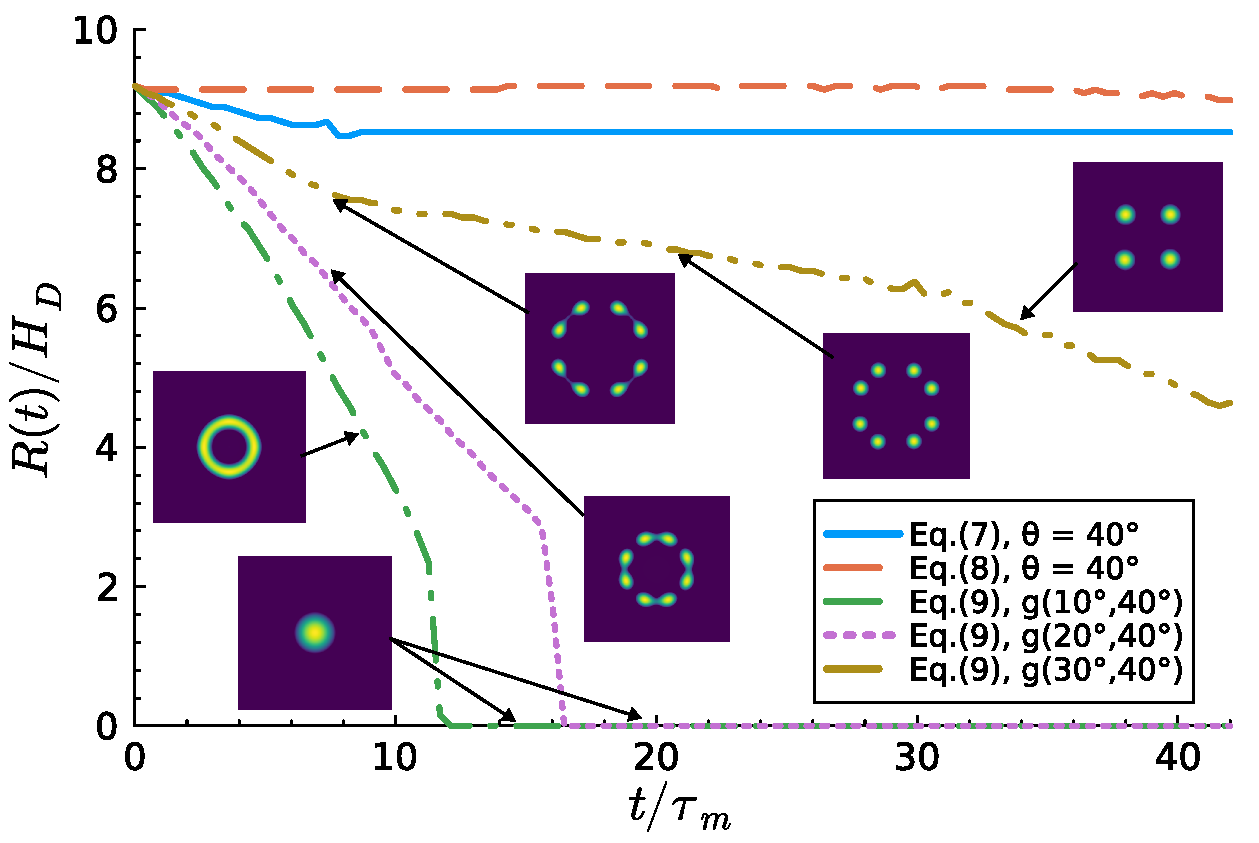
\includegraphics[width=0.48\textwidth]{assets/grad_heatmap.pdf}
    \caption{Evolution of the radius of a ring-rivulet $R(t)$ normalized by the droplet height $H_D$ for different contact angle cases (line styles and colours) and $\psi = 0.133$.
    The first argument of $g(a,b)$ is the contact angle in the centre of the numerical domain and the second argument is the contact angle at $R_0$ and beyond. 
    Besides the lines we add heatmap snapshots of the film thickness $h(\mathbf{x},t)$ where yellow indicates a large value and dark blue a small value (colorbars are not scaled).}
    \label{fig:negativewetgrad}
\end{figure}
As the last part of this section we want to address the impact of a linear wettability gradient on the dynamics of the ring-rivulet. 
We first consider a positive wettability gradient, thus the wettability increases towards the centre of the domain starting from $R_0$ and is kept constant for $\xi > R_0$.
Fig.~\ref{fig:negativewetgrad} shows measurements of the ring radius $R(t)$ for different wettability scenarios with $\psi_0 = 0.133$.
The different colours depict different simulations, including the uniform substrate and the banded pattern shown in blue and orange respectively.
These two line show only a minor change in $R(t)$ and then appear to be stationary.
Which can be explained by the fact that the ring ruptures and forms droplets, these droplets do not move and therefore $R(t)$ does not change.
On the other hand the remaining three curves show the impact of a wettability gradient.  
In green we have the highest wettability gradient, starting from $\theta = 40^{\circ}$ at $\xi = R_0$ decreasing to $\theta = 10^{\circ}$ at $\xi = 0$. 
The dynamical evolution of the ring-rivulet is clearly different from the uniform and banded case.
Instead of a breakup we see a constant contraction and the ring remains stable until a single droplet is formed at the centre of the substrate.
While the radius of that droplet is not zero we made the arbitrary choice to set $R(t) = 0$ if the liquid-solid area is a disk, inline with the topological change and the switch of the Euler characteristic $\chi$ from 0 to 1.
We see that a wettability gradient can transform an initial condition that would break up into a collapsing one.

Even more interesting are the two remaining curves, thus the purple and golden one.
From green to golden the wettability gradient becomes smaller, going from a $30^{\circ}$ difference to a $10^{\circ}$ difference.
The purple is in between the green and the golden with a $20^{\circ}$ difference. 
Similar to the green one we see a linear change in $R(t)$ with a kink shortly before a single droplet is formed.
However, in this case the ring-rivulet is breaking up and forms four intermediate droplets, as shown with heatmaps in Fig.~\ref{fig:negativewetgrad}.
Due to the wettability gradient these droplets are not stationary, but are advected towards the centre of the substrate and form a single droplet on a slightly longer time scale as compared to the green curve.
The golden curve has the smallest wettability gradient which effectively deceleration the dynamics.
Similar to the purple one the rivulet breaks up, but it forms eight droplets instead of four, similar to the uniform substrate.
Again the droplets are advected towards the centre of the substrate, but as the gradient is smaller the radius changes on longer time scales. 
Around $t\approx 32\tau_m$ the two droplets closest to each other coalesce and after $t\approx 35\tau_m$ we only have four droplets.
The final state again would be a single droplet in the centre of the substrate.

\begin{figure}
    \centering
    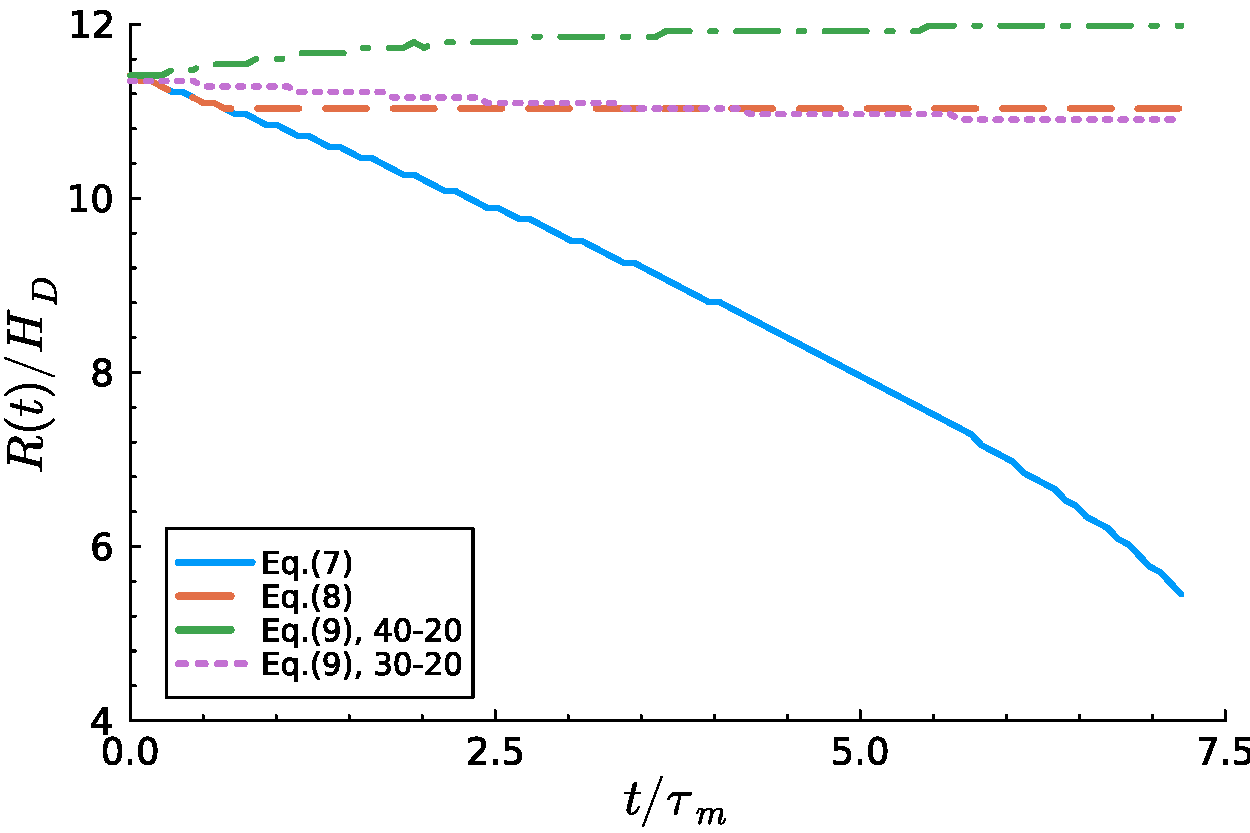
\includegraphics[width=0.48\textwidth]{assets/radius_time_gradient_positive.pdf}
    \caption{Evolution of the radius of a ring-rivulet $R(t)$ normalized by the droplet height $H_D$ for different contact angle cases (line styles and colours) and $\psi = 0.3$.
    The first argument of $g(a,b)$ is the contact angle in the centre of the numerical domain and the second argument is the contact angle at $R_0$ and beyond.}
    \label{fig:positivewetgrad}
\end{figure}
A wettability gradient, therefore, allows us to alter the time scales $t_b$ and $t_c$.
For the smallest positive gradient, the golden curve, we are in fact able to switch between an eight, four and one droplet state simply be means of the radial gradient. 
For completeness we then performed numerical experiments with a negative wettability gradient, thus the centre of the substrate is less wettable than the rest.
In Fig.~\ref{fig:positivewetgrad} we show $R(t)$ data of four simulations with $\psi_0 = 0.3$.
The blue curve depicts the evolution on the uniform substrate, as indicated in Fig.~\ref{fig:max_drops} $\psi_0$ values larger than $0.25$ lead to a collapse.
Unsurprisingly, the banded pattern prohibits this collapse and stabilizes the ring during the duration of the numerical experiment as shown by the orange dashed line.
Additionally we have two negative gradients shown in green and purple. 
The larger negative gradient, the green curve, the centre of the rivulet is actually pushed away from $R_0$ leading to an increase of radius.
Here we also observe a break up in the long time limit, due to the use of periodic boundary conditions we observe the coalescence of two droplets and thus only have three droplets.
Without periodic boundary conditions we most likely find four droplets which would agree with Eq.~(\ref{eq:maxDrops}).
For the smaller negative gradient we do not observe such an effect and the data is barely distinguishable from the banded case.
In neither of these two case we see a break up until the last iteration of our simulation.
However, once again a wettability gradient changes a collapsing state into a non collapsing one.

\section{Conclusions}\label{sec:conclu}
We have presented numerical experiments of a liquid ring-rivulet on a uniform and patterned substrate. 
The basis of our experiments is the thin film equation with a disjoining pressure model.
We are able to reproduce results of Gonz{\'a}lez et al.~\cite{gonzalezStabilityLiquidRing2013} and show some agreement for small $\psi_0$ values concerning the most unstable mode and as such the number of droplets, for both the uniform and a patterned substrate.
For $\psi_0 > 0.25$ the capillary retraction outpaces the breakup and the collapse is the more likely outcome.
We further found a good analytical approximation for the growth rate on the uniform substrate as shown in Fig.~\ref{fig:first_growth}. 

Our main aim, however, is to address the impact of wettability on the dynamics of the ring-rivulet.
We therefore considered two patterns, one that restricts the rivulet to a band and effectively removes the collapse mode and a positive as well as a negative wettability gradient towards the centre.
The banded pattern shows good agreement with the predicted number of droplets, in the small $\psi_0$ regime. 
Interestingly, the rupture times seems linearly correlated with $\psi_0$ as shown in Fig.~\ref{fig:bandBreakupT}.

The wettability gradient patterns on the other hand allow us to tune the two competing time scales, namely the breakup time $t_b$ and the collapse time $t_c$.
We show this in Fig.~\ref{fig:negativewetgrad}, where the initial conditions ($\psi \approx 0.13$) favor a breakup of the ring, or $t_b < t_c$.
By applying the positive wettability gradient we can not only force the rivulet to end up in a collapsed state, but can approach this state via different trajectories. 
Having a strong radial gradient allows to skip the breakup and thus $t_c < t_b$.
If we however the gradient we can pass by different droplet states with either four or eight droplets.
In case of a negative radial wettability gradient we find that similar to the band pattern, collapse is unlikely.

As a future perspective of this work we would like to add thermal fluctuations to the system as some experimental realizations using molten metal.
On the other hand a dynamic pattern may allow for radial breakup as well, because currently we only observed azimuthal breakup.

\section*{Author Contributions}
We strongly encourage authors to include author contributions and recommend using \href{https://casrai.org/credit/}{CRediT} for standardised contribution descriptions. Please refer to our general \href{https://www.rsc.org/journals-books-databases/journal-authors-reviewers/author-responsibilities/}{author guidelines} for more information about authorship.

For footnotes in the main text of the article please number the footnotes to avoid duplicate symbols. \textit{e.g.}\ \texttt{\textbackslash footnote[num]\{your text\}}. The corresponding author $\ast$ counts as footnote 1, ESI as footnote 2, \textit{e.g.}\ if there is no ESI, please start at [num]=[2], if ESI is cited in the title please start at [num]=[3] \textit{etc.} Please also cite the ESI within the main body of the text using \dag. For the reference section, the style file \texttt{rsc.bst} can be used to generate the correct reference style.

\section*{Conflicts of interest}
There are no conflicts to declare.

\section*{Acknowledgements}
S. Z. and J. R. acknowledge the financial support from the Independent Research Fund Denmark through a DFF Sapere Aude Research Leader grant (grant number 9063-00018B).



%%%END OF MAIN TEXT%%%

%The \balance command can be used to balance the columns on the final page if desired. It should be placed anywhere within the first column of the last page.

\balance

%If notes are included in your references you can change the title from 'References' to 'Notes and references' using the following command:
%\renewcommand\refname{Notes and references}

%%%REFERENCES%%%
\bibliography{rsc} %You need to replace "rsc" on this line with the name of your .bib file
\bibliographystyle{rsc} %the RSC's .bst file

\appendix
\section{Numerical model and parameters}\label{app:numerics}
The numerical model is based on a single relaxation (SRT) time lattice Boltzmann method. 
The relaxation time $\tau$ is set to $\tau = 1$ in all our numerical experiments. 
This means that the fluid's kinematic viscosity $\nu$ is set to $\nu = 1/6$ and kept constant for all simulations.  


The surface tension $\gamma$ is set to $\gamma = 10^{-2}$ for all results presented here.
We did in fact simulate with different values of $\gamma$ but found that the effect is an overall rescaling of the time scale, larger $\gamma$ speeds up all dynamics, lower $\gamma$ values slows them down.

Lastly $\alpha_{\delta}(h)$ is a substrate friction term that mimics a slip boundary condition with an effective slip length $\delta$
\begin{equation}\label{eq:alphafric_app}
\alpha_{\delta}(h) = \frac{6h}{(2 h^2 + 6 \delta h + 3 \delta^2)}.
\end{equation}
By introducing a precursor layer $h_{\ast}$ and a slip length $\delta$ we regularize the contact line divergence~\cite{huhHydrodynamicModelSteady1971}. 
The slip length lies within the weak/intermediate slip regime~\cite{peschkaSignaturesSlipDewetting2019,fetzerQuantifyingHydrodynamicSlip2007, munchLubricationModelsSmall2005} and the thickness of the precursor film is set to $h_{\ast} = 0.05$.

By applying this solution for $\mathbf{u}$ to the continuity equation we have
\begin{equation}\label{eq:thinsolve_app}
     \partial_t h(\mathbf{x},t) = \nabla\cdot\left(M_{\delta}(h)\nabla p_{\mbox{\tiny{film}}}\right),
\end{equation}
with the mobility function $M_{\delta}(h) = \frac{h^2}{\mu\alpha_{\delta}(h)}$ which for the no-slip boundary condition $(\delta \rightarrow 0)$ reduces to $M_{0}(h) = h^3/3\mu$.
Without loss of generality we set $\rho_0 = 1$ and thus the dynamic viscosity is $\mu = \rho_0 \nu = 1/6$. 

The numerical domain consists of a square lattice with $512\Delta x$ in both horizontal directions.
We further use biperiodic boundary conditions at the edges of the domain. 





\end{document}
